\documentclass[a4paper,10pt]{scrartcl}

\usepackage{standalone}

% Load ``float'' before ``hyperref`` before ''algorithm``
% Note: ''algorithm`` would load ''float`` by itself
\usepackage{float}
\usepackage[pagebackref,hyperindex=true]{hyperref}

%%%%%%%%%%%%%%%%%%%%%%%%%%%%
% Math
%%%%%%%%%%%%%%%%%%%%%%%%%%%%
\usepackage{amsmath}
\usepackage{amssymb}
\usepackage{amsfonts}
\usepackage{amsopn}
\usepackage{braket}
\usepackage{bbm}
\usepackage{dsfont}
% \usepackage{mathabx}


% Various new commands that ease typesetting math even further
% \newcommand{\assign}{\ensuremath{\coloneq}}
% \newcommand{\rassign}{\ensuremath{\eqcolon}}
% TODO: remove
% \newcommand{\assign}{\ensuremath{:=}}
% \newcommand{\rassign}{\ensuremath{=:}}
% \newcommand{\seteq}{\ensuremath{\overset{!}{=}}}
% \newcommand{\of}[1]{\ensuremath{\left( #1 \right)}}
% \newcommand{\ofs}[1]{\ensuremath{\left( #1 \right)}}
% \newcommand{\norm}[1]{\ensuremath{\| #1 \|}}
% \newcommand{\tmop}[1]{\ensuremath{\operatorname{#1}}}
% \newcommand{\id}{\ensuremath{\mathds{1}}}
% % \newcommand{\id}{\ensuremath{I}}
% \newcommand{\kron}[1]{\ensuremath{\delta_{#1}}}
% \newcommand{\conj}[1]{\ensuremath{\overline{#1}}}
% \renewcommand{\vec}[1]{\ensuremath{\underline{#1}}}
% \newcommand{\mat}[1]{\ensuremath{\mathbf{#1}}}
% \newcommand{\inv}{\ensuremath{{}^{-1}}}
% \newcommand{\T}{\ensuremath{{}^{\textnormal{T}}}}
% \renewcommand{\H}{\ensuremath{{}^{\textnormal{H}}}}
% \newcommand{\Tinv}{\ensuremath{{}^{\textnormal{-T}}}}
% \newcommand{\Hinv}{\ensuremath{{}^{\textnormal{-H}}}}
% \newcommand{\tr}{\ensuremath{\textnormal{Tr}}}
% \newcommand{\ft}[1]{\ensuremath{\mathcal{F}\left(#1\right)}}
% \newcommand{\ift}[1]{\ensuremath{\mathcal{F}^{-1}\left(#1\right)}}
% \newcommand{\fft}[1]{\ensuremath{\mathtt{FFT}\left(#1\right)}}
% \newcommand{\ifft}[1]{\ensuremath{\mathtt{IFFT}\left(#1\right)}}
% \newcommand{\dotp}[2]{\ensuremath{\left\langle #1 , #2 \right\rangle}}
% \newcommand{\bigO}[1]{\ensuremath{\mathcal{O}\left( #1 \right)}}
% \newcommand{\laplace}{\ensuremath{\operatorname{\Delta}}}
% \newcommand{\diff}[3][]{\frac{\mathrm{d}^{#1}#2}{\mathrm{d}#3^{#1}}}
% \newcommand{\pdiff}[3][]{\frac{\partial^{#1}#2}{\partial #3^{#1}}}

%%%%%%%%%%%%%%%%%%%%%%%%%%%%
% Graphics
%%%%%%%%%%%%%%%%%%%%%%%%%%%%
\usepackage{graphicx}
\usepackage{subfig}
\usepackage{asymptote}
\usepackage{tikz}
\usetikzlibrary{topaths,calc}
\usetikzlibrary{positioning}
\usetikzlibrary{arrows,shapes,backgrounds}
\definecolor{gray}{gray}{0.55}


%%%%%%%%%%%%%%%%%%%%%%%%%%%%
% Math
%%%%%%%%%%%%%%%%%%%%%%%%%%%%
\usepackage{algorithm}
% \usepackage{algorithmic}
\usepackage{color}
\usepackage{relsize}
\usepackage[scaled=0.8]{beramono}

%%%%%%%%%%%%%%%%%%%%%%%%%%%%
% Code
%%%%%%%%%%%%%%%%%%%%%%%%%%%%
\usepackage{listings}
% C++ Code macro
\newcommand{\cpp}[1] {
  \lstset{language=c++,
          basicstyle=\smaller,
          basewidth=0.58em,
          columns=fixed,
          tabsize=2,
          fontadjust=true,
          frame=l,
          xleftmargin=4.2pt,
          numbers=left,
          stepnumber=2,
          breaklines=true,
          breakindent=0pt,
          prebreak=\mbox{\tiny$\searrow$},
          postbreak=\mbox{{\color{gray}$\cdots$}},
          numberstyle=\color{gray},
          commentstyle=\color{gray},
          stringstyle=\textit,
          showstringspaces=false,
        }
  \lstinputlisting{#1}
}
  
  \lstset{language=c++,
          basicstyle=\smaller,
          basewidth=0.58em,
          columns=fixed,
          tabsize=2,
          fontadjust=true,
          breaklines=true,
          breakindent=0pt,
          prebreak=\mbox{\tiny$\searrow$},
          postbreak=\mbox{{\color{gray}$\cdots$}},
          numberstyle=\color{gray},
          commentstyle=\color{gray},
          stringstyle=\textit,
          showstringspaces=false,
          basicstyle=\footnotesize
        }


%%%%%%%%%%%%%%%%%%%%%%%%%%%%
% More Packages
%%%%%%%%%%%%%%%%%%%%%%%%%%%%
\usepackage[utf8x]{inputenc}
\usepackage{cancel}
\usepackage{url}
\usepackage{placeins}
\usepackage{microtype}
\usepackage{amsthm}
\newtheorem{theorem}{Theorem}
\newtheorem{definition}{Definition}

% Links in pdf
\usepackage{color}
\newcommand{\blue}{ \color{blue} }
\definecolor{linkcol}{rgb}{0,0,0.4}
\definecolor{citecol}{rgb}{0.5,0,0}

\hypersetup
{
colorlinks=true,
linkcolor=linkcol,
citecolor=citecol,
urlcolor=linkcol
}

% nicer backref links
\renewcommand*{\backref}[1]{}
\renewcommand*{\backrefalt}[4]{%
\ifcase #1 %
(Not cited.)%
\or
(Cited on page~#2.)%
\else
(Cited on pages~#2.)%
\fi}
\renewcommand*{\backrefsep}{, }
\renewcommand*{\backreftwosep}{ and~}
\renewcommand*{\backreflastsep}{ and~}

% TODO: set some indent
% \parindent 0cm

\newcommand{\clearemptydoublepage}{\newpage{\pagestyle{empty}\cleardoublepage}}


% Mycommands

\usepackage{bm}

% \newcommand*{\op}[1]{\hat{\mathcal{#1}}}
\newcommand*{\C}{\ensuremath{\mathbb{C}}}
\newcommand*{\Dt}{\ensuremath{\Delta t}}
\newcommand*{\K}{\ensuremath{\mathcal{K}}}
\newcommand*{\R}{\ensuremath{\mathbb{R}}}
\newcommand*{\bmat}[1]{\bm{#1}}
\newcommand*{\bvec}[1]{\bm{#1}}
\newcommand*{\conj}[1]{\overline{#1}}
\newcommand*{\del}{\ensuremath{\partial}}
\newcommand*{\dif}{\ensuremath{d}}
\newcommand*{\dt}{\ensuremath{\delta t}}
\newcommand*{\eps}{\ensuremath{\varepsilon}}
\newcommand*{\im}{\ensuremath{\imath}}
\newcommand*{\opH}{\mathcal{H}}
\newcommand*{\opT}{\mathcal{T}}
\newcommand*{\opU}{\mathcal{U}}
\newcommand*{\opV}{\mathcal{V}}
\newcommand*{\opW}{\mathcal{W}}
\newcommand*{\opA}{\mathcal{A}}
\newcommand*{\opB}{\mathcal{B}}
\newcommand*{\opX}{\mathcal{X}}
\newcommand*{\upic}{\ensuremath{u[\Pi,\bm{c}]}}
\newcommand*{\proc}[1]{\textsc{#1}}

\usepackage{algorithm}
\usepackage{verbatim}
\usepackage{physics}
\usepackage{amssymb}
\usepackage{bm}
% \usepackage[noend]{algpseudocode}
\usepackage{algpseudocode}


\usepackage{tikz}
\usetikzlibrary{arrows,chains,matrix,positioning,scopes}
\usepackage{multicol}


\begin{document}

\begin{titlepage}
	\begin{center}

		\hfill

		\vspace{2cm}

		{\huge \textsc{Time Propagation\\ of Quantum Wave Packets\\[10pt]}}
		{\Large \textsc{an efficient implementation in C++\\[10pt]}}

		\vspace{1cm}

		{\Large{Bachelor Thesis}}

		\vspace{1cm}

		{\emph{written by}} \\
		{
			Matthias Untergassmair
		}

		\vspace{1cm}

		{\emph{advised by}} \\
		{
			Raoul Bourquin
		}

		\vspace{1cm}

		{\emph{supervised by}} \\
		{
			Dr. Vasile Gr\u{a}dinaru\\
			Prof. Dr. Ralf Hiptmair
		}
		
		\vfill

		Seminar for Applied Mathematics\\
		ETH Zurich

		\vspace{.5cm}

		\emph{{Fall semester 2016}}

		\vspace{.5cm}

		
\includegraphics[width=0.5\linewidth]{figures/eth-logo.pdf}

	\end{center}

\end{titlepage}


\clearemptydoublepage

\mbox{}
\vfill
\begin{abstract}
	This article explains the central design decisions and most important code details related to the efficient implementation of time propagation for Hagedorn wave packets in the WaveBlocks framework.
	A short introduction to operator splitting and a summary of some of the most important time propagation schemes for Hagedorn wave packets are also given.
	Finally, some benchmarking results are presented which analyze energy conservation and compare different propagators, splitting schemes, step sizes and dimensionalities.
\end{abstract}

\vfill
\tableofcontents

\clearpage

\listoffigures
\listofalgorithms

\clearemptydoublepage

% \section*{Introduction}
%
With the growing understanding for quantum mechanics and quantum dynamics, one can attempt to solve increasingly complex systems and computational problems.
Without doubt, time propagation is at the core of simulating quantum systems and getting a better understanding for them.
\par\medskip
%
The aim of this project was to give a summary of some state of the art quantum time propagators and provide an efficient C++ implementation for evolving Hagedorn wave packets in time.
The produced code is an addition to the C++ WaveBlocks Framework whose functionality has already been extended in the context of preceding student projects.
The entire WaveBlocks project, which is partially based on an existing Python project with the same name, can be found at \cite{libwaveblocks}.
\par\medskip
%
In this report, section \ref{sec:operatorsplitting} repeats some of the most important mathematical ideas underlying the time propagation of wave packets and introduces the notations that will be used throughout the rest of the document.
Based on these mathematical observations, section \ref{sec:buildingblocks} prepares a toolbox of essential building blocks that will help in the construction of propagators as well as for the final understanding of the source code.
In section \ref{sec:propagators}, a series of numerical propagators for quantum wave packets are presented and expressed in terms of the components provided earlier.
Some detailed insights into the most important technical ideas of the C++ implementation are given in section \ref{sec:implementation}.
Finally, section \ref{sec:results} presents the results of a series of numerical experiments to show the correctness of the implemented algorithms and analyse some performance aspects like the scaling with step size, dimensionality of the wave packet and order of the splitting coefficients.

% \input{./wavefunction_propagation.tex}
% \input{./wavepackets.tex}
% \input{./observables.tex}
% \input{./wavepacket_propagation.tex}
% \section{Results}
\label{sec:results}
%
The newly developed code was used to carry out some numerical experiments which are presented in this section.
Aspects that need to be checked are the correctness of the propagators from a quantum mechanical point of view (subsection~\ref{subsec:physical}), convergence of the methods (subsection~\ref{subsec:convergence}) and benchmarking of the compute time (subsection~\ref{subsec:benchmark}).

\subsection{Physical Correctness}
\label{subsec:physical}
{\Huge TODO: Review this part}
%
In order to analyze the physical correctness of the implemented propagators, a two dimensional wave packet was propagated with each of the presented propagators for a time $T = 10$ with timestep $\Dt = 0.01$.
All propagators used the \emph{Y4} splitting coefficients for the \proc{IntSplit} method.
\par\medskip
%
The harmonic potential was used as an example potential as it is easy to verify.
The generalized harmonic potential for $D$ dimensions is
\begin{align}
	V(\bvec{x}) = 
	\frac{1}{2} \sum_{i=1}^D x_i^2
\end{align}
%
where $x_i, \; 1 \le i \le D$ denote the single entries of the vector $\bvec{x}$.
\par\medskip
%
Figure \ref{fig:energy_Semiclassical} shows the time evolution of energy and the energy drift for the semiclassical propagator. The corresponding energy plots for the remaining propagators can be found in the appendix to the report. \\
As is clearly shown by the graphs, the propagators conserve the total energy (apart from very small oscillations of the order $10^{-7}$ for the Hagedorn propagator and $10^{-12}$ for the remaining propagators that use \proc{IntSplit}).
Another interesting fact is that the \emph{McL84} operator seems to have a much longer oscillation period than all other propagators.
%
\begin{figure}[ht]
	\centering
	\begin{minipage}[c]{\textwidth}
		\begin{center}
			\large Semiclassical Propagator \\[1mm]
			\normalsize Energy Evolution and Drift
			\vspace{4mm}
		\end{center}
	\end{minipage}
	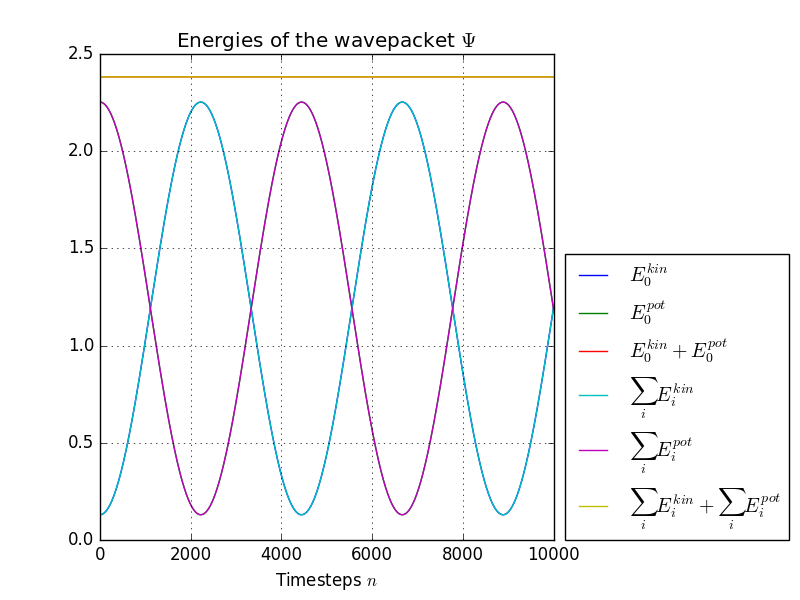
\includegraphics[width=.45\textwidth]{figures/energy_Semiclassical.png}
	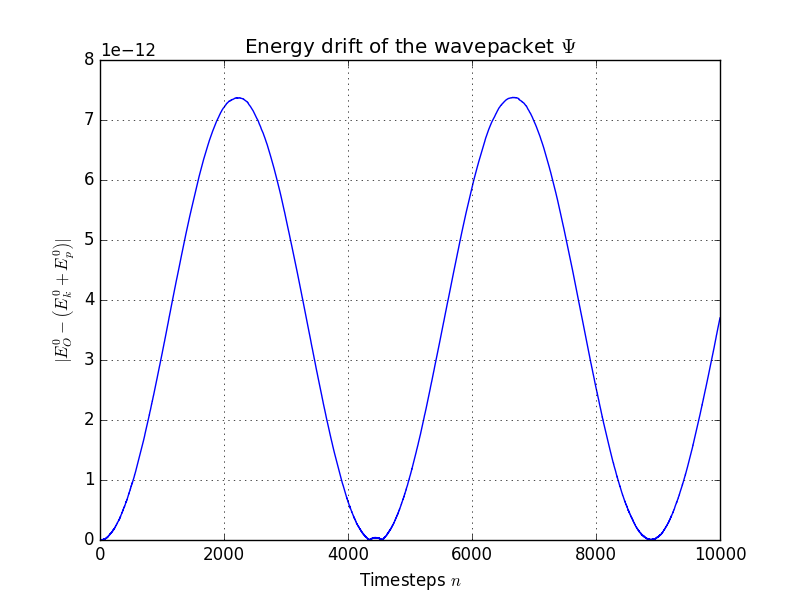
\includegraphics[width=.45\textwidth]{figures/drift_Semiclassical.png}
	\caption{Energy Evolution and Drift for a 2D Wave Packet evolved for $T = 10$ with step $\Dt = 0.001$ in a harmonic potential using the Semiclassical Propagator with \emph{Y4} splitting}
	\label{fig:energy_Semiclassical}
\end{figure}


\subsection{Effect of Stepsize}
\label{subsec:convergence}
{\Huge TODO: Review this part}
%
A convergence analysis was carried out in which the error of each propagator was recorded while reducing the stepsize.
A Semiclassical propagator with \emph{KL10} splitting coefficients and step size 0.001 was used to propagate the wave packet to a final time $T = 10$ and create a reference solution.
\par\medskip
%
The error between two wave packets was computed by evaluating them on a grid with 1000 grid points and taking the $L_2$ norm of the differences.
Figure \ref{fig:error_analysis} shows the error for different step sizes $\Dt$.
It is quite surprising how the Hagedorn Propagator seems to have even better convergence order than all the more sophisticated contestants.
Also, the \emph{McL84} propagator does not seem to converge. This is consistent with the observation made earlier in this section that - although satisfying energy conservation - the \emph{McL84} propagator seemed to have a vastly different period of oscillation.
%
{\Huge TODO: Review this part}
%
\begin{figure}[ht]
	\centering
	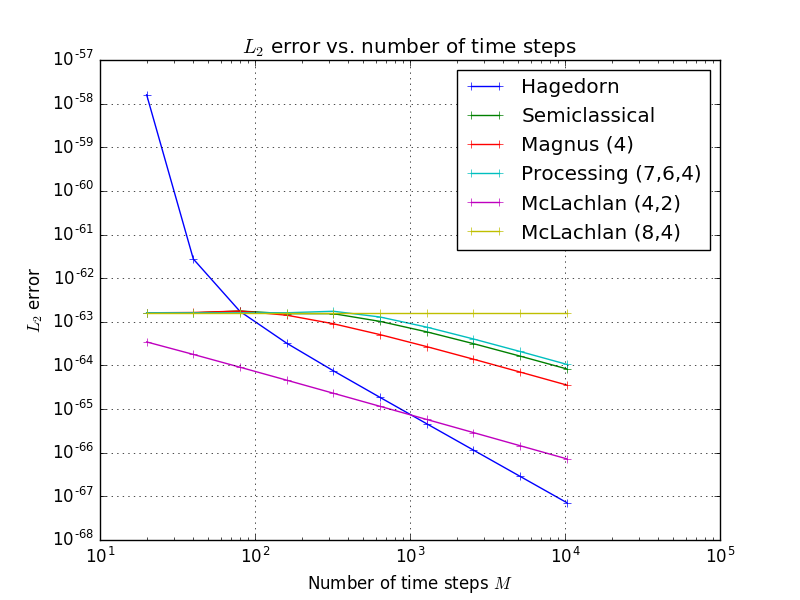
\includegraphics[width=.8\textwidth]{figures/error_analysis.png}
	\caption{Convergence of the wavefunctions towards the reference solution. The $L_2$ norm was measured by projecting the wave function on a grid with 1000 nodes in the range $[-1,1]$ and taking the differences of these values. According to this experiment, the Hagedorn propagator seems to have higher convergence order than its contestants, despite its simplicity.
	This observation could be an interesting starting point for further experiments.}
	\label{fig:error_analysis}
\end{figure}

\subsection{Benchmark}
\label{subsec:benchmark}
%
In order to benchmark the code, three timing experiments were carried out: a simple comparison of runtimes for different propagators, an investigation of the computational cost associated with the usage of high order splitting schemes, and an analysis of the compute time as a function of the dimension $D$.
In all cases, the harmonic potential introduced at the beginning of this section was used.
\par\medskip
%
The runtime analysis was carried out on a Linux (Kernel 4.8.7, Fedora 24 Workstation) Quad-Core machine with an Intel Core i5-3210M Processor and
4GB of RAM. The C++ code was compiled with the GNU compiler, version 6.2.1, and using the \emph{-Ofast} optimization flag.




\subsubsection{Comparison of propagators}
%
A quick comparison of timings for the different propagators is shown in table \ref{tab:speedup}.
The same setup as for the energy analysis was used (2D wave packet, $T = 10$, step size $\Dt = 0.001$, \emph{Y4} time splitting coefficients).
It comes as quite a surprise, that the Semiclassical propagator is faster at computing the result than the Hagedorn propagator, which at first glance seems to have  a simpler structure and involve fewer steps.
Also, the Magnus Propagator \emph{MG4} is cheaper than expected, as it involves two evaluations of $\matrixel{\varphi_k}{W}{\varphi_l}$ per time step but is only slightly slower than the Semiclassical operator with one evaluation of the inner product.
%
\begin{table}[ht]
	\centering
	\begin{tabular}{|l | r |} 
		\hline
		\multicolumn{1}{|c}{\textbf{Propagator}} &
		\multicolumn{1}{|c|}{\textbf{Timing [s]}} \\
		\hline
		Hagedorn & 12.54 \\
		Semiclassical & 12.51 \\
		MG4 & 13.82 \\
		Pre764 & 17.10 \\
		McL42 & 22.82 \\
		McL84 & 23.52 \\
		\hline
	\end{tabular}
	\caption{Runtimes for propagating a 2D wave packet to a time $T = 10$ with timestep $\Dt = 0.001$ with different propagators in C++. All the timings in the table were measured by taking the average of 10 independent runs. The standard deviation of these measurements was below $0.1\%$.}
	\label{tab:speedup}
\end{table}


\subsubsection{Splitting Schemes}
%
As mentioned previously, the splitting coefficients $\{ w_T, w_U \}$ that are used as weights on the timestep $\dt$ in the \proc{IntSplit} method can have vastly different complexity, ranging from the \emph{Lie-Trotter} coefficients (one coefficient for propagation with $\opT$, one for propagation with $\opU$) up to the \emph{KL10} coefficients (34 coefficients for each operator). \\
Higher order schemes are usually preferred in terms of accuracy, but they come at the price of longer computation time.
\par\medskip
%
Therefore, a numerical experiment was carried out in order to analyze how much computational time is consumed for coefficient pairs of different sizes.
In order to create a reference solution, the Semiclassical Propagator was used to propagate a two dimensional wave packet in a harmonic potential over a time of $T = 400$ and with stepsize $\Dt = 0.01$.
The same simulation was carried out for coefficient pairs of various different sizes and were run in Python as well as C++.
The results are listed in table \ref{tab:benchmarksplit_t} and plotted in figure \ref{fig:benchmarksplit_f}.
\par\medskip
%
Looking at the Python timings only, the measurements suggest that in the case of the \emph{KL10} coefficient set, at least 80\% of the total runtime is spend in the \proc{IntSplit} function (since larger coefficient sets $\{ w_T, w_U \}$ only affect the number of steps with operators $\opT$ and $\opU$, but not with operator $\opW$).
\par\medskip
%
When bringing the timings in context with the C++ code, a comparison of absolute runtimes is of course not fair since C++ is intrinsically faster than a scripting language like Python and the C++ version has been optimized for speed in many different ways.
However, a very significant result in the context of the work on Propagators is how the speedup increases for larger coefficient pairs.
Using the \emph{KL10} coefficient set instead of a simple \emph{LT} set, the Python code takes more than six times longer.
The same comparison on C++ code shows that the code takes only 30\% longer for the large coefficient set than it takes for the minimal coefficient set.
This is a very encouraging result as it means that high order splitting coefficients come at almost no extra cost.
\par\medskip
%
\begin{table}[ht]
	\centering
	\begin{tabular}{|l | r | r | r | r |} 
		\hline
		\multicolumn{1}{|c}{\textbf{Splitting}} &
		\multicolumn{1}{|c}{\textbf{No. of coefs}} &
		\multicolumn{1}{|c}{\textbf{Python timing [s]}} &
		\multicolumn{1}{|c}{\textbf{C++ timing [s]}} &
		\multicolumn{1}{|c|}{\textbf{Speedup}} \\
		\hline
		LT & 1 & 174.6 & 5.766 &\textbf{30.3} \\ 
		S2 & 2 & 202.9 & 5.706 &\textbf{35.6} \\
		Y4 & 4 & 258.6 & 5.861 &\textbf{44.1} \\
		PRKS6 & 7 & 341.0 & 5.995 &\textbf{56.9} \\ 
		Y61 & 8 & 366.0 & 6.004 &\textbf{61.0} \\
		KL6 & 10 & 421.4 & 6.124 &\textbf{68.8} \\
		BM63 & 15 & 557.1 & 6.467 &\textbf{86.2} \\ 
		KL8 & 18 & 634.8 & 6.637 &\textbf{95.6} \\
		KL10 & 34 & 1067.2 & 7.457 &\textbf{143.1} \\
		\hline
	\end{tabular}
	\caption{Table comparing the computation time of Python code vs. C++ code for different sizes of the splitting coefficients $\{ w_T, w_U \}$. All the timings in the table were measured by taking the average of 10 independent runs. The standard deviation of these measurements was below $1\%$ for the Python timings and below $0.1\%$ for the C++ timings.}
	\label{tab:benchmarksplit_t}
\end{table}
%
\begin{figure}[ht]
	\centering
	\begin{center}
	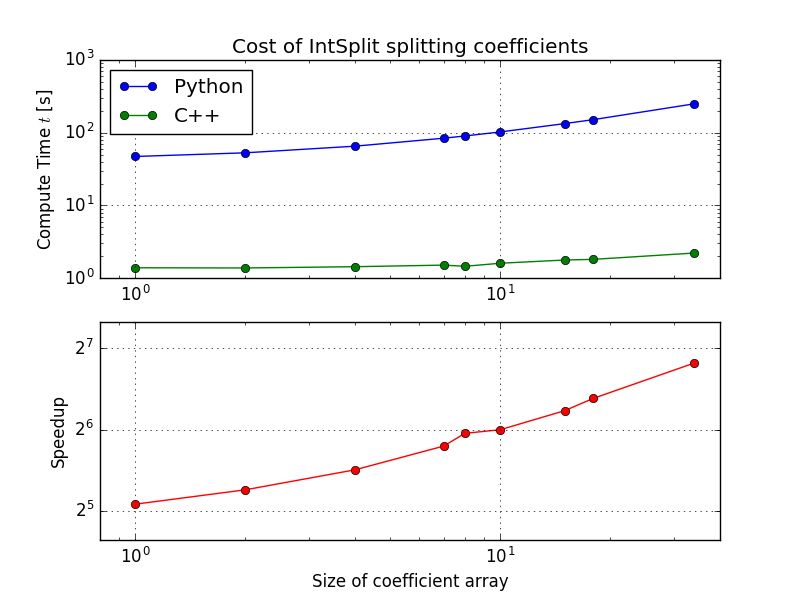
\includegraphics[width=.8\textwidth]{figures/coefficient_analysis.png}
	\end{center}
	\caption{Comparison of computation times for different splitting coefficients $\{ w_T, w_U \}$. The absolute timings are shown in the top graph, the speedup on the bottom. It is remarkable that the initial speedup factor is about 30, but grows for larger coefficient sets. The speedup factor for the largest tested coefficient pair \emph{KL10} is over 140.}
	\label{fig:benchmarksplit_f}
\end{figure}


\subsubsection{Scaling with dimensionality D}
%
The question that was addressed in this benchmark is how the compute time of the code scales with increasing dimension $D$ of the wave packet.
Figure \ref{fig:dimension_analysis} shows a clear exponential scaling with the dimension $D$.
With a computation time of under 20 minutes for 100 time steps with the Semiclassical Propagator, dimension $D=5$ is still quite feasible.
%
\begin{figure}[ht]
	\centering
	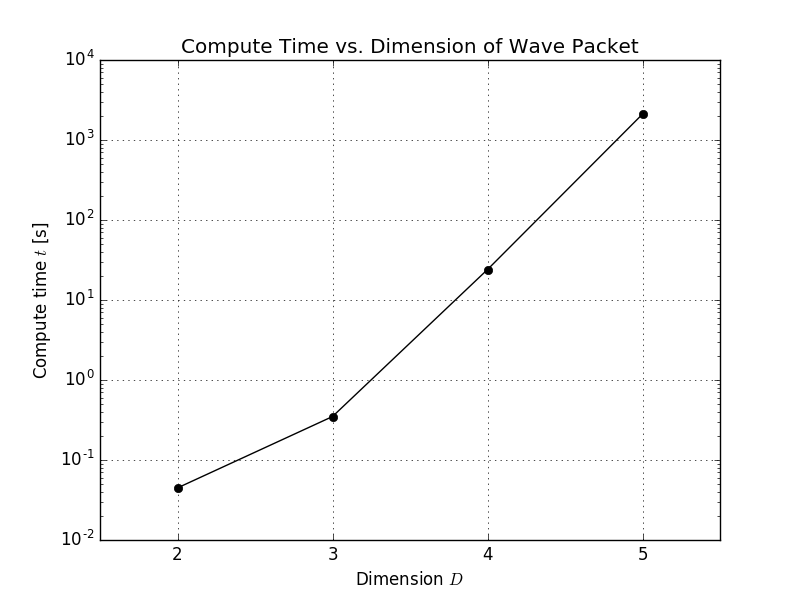
\includegraphics[width=.8\textwidth]{figures/dimension_analysis.png}
	\caption{Scaling of the computation time with wave packet dimension $D$. Measurements done for a wave packet in a generalized harmonic potential, propagated for 100 steps with the Semiclassical Propagator.}
	\label{fig:dimension_analysis}
\end{figure}




%%%%%%%%%%%%%%%%%%%%%%%%%%%%%%%%%%%%%%%%%%%%%%%%%%%%%%%%%%%%%%%%%%%%%%%%%%%%%%%%%%%%%
%%%%%%%%%%%%%%%%%%%%%%%%%%%%%%%%%%%%%%%%%%%%%%%%%%%%%%%%%%%%%%%%%%%%%%%%%%%%%%%%%%%%%
%%%%%%%%%%%%%%%%%%%%%%%%%%%%%%%%%%%%%%%%%%%%%%%%%%%%%%%%%%%%%%%%%%%%%%%%%%%%%%%%%%%%%

% TODO: move to separate file when done

%%%%%%%%%%%%%%%%%%%%%%%%%%%%%%%%%%%%%%%%%%%%%%%%%%%%%%%%%%%%%%%%%%%%%%%%%%%%%%%%%%%%%

\clearpage
\section{Introduction}

All based on composition methods

methods that compose elementary flows/operators to build an approximation of high order

In general / in the practical implementation, propagation with $\opT$ and $\opU$ is usually replaced by a series of smaller, alternating steps with the two operators


Summary of the structure of the remaining report
%%%%%%%%%%%%%%%%%%%%%%%%%%%%%%%%%%%%%%%%%%%%%%%%%%%%%%%%%%%%
\cite{GH_convsemiclassical}
Semiclassical time-dependent Schrödinger equation
%
\begin{align}
	\label{math:tdse}
	\im \eps \; \del_t \psi (\bvec{x},t) = \opH (\eps) \; \psi (\bvec{x},t)
\end{align}
%
with wave function $\psi(\bvec{x},t)$ depending on the spatial variables $\bvec{x} = (x_1,\dots,x_D) \in \R^D$ and the time variable $t \in \R$.

Hamiltonian
\begin{align}
	\opH = \opT + \opV = \opT + \opU + \opW
\end{align}
\begin{align}
	\opT &= - \sum_{j=1}^D \frac{\eps^2}{2m_j} \frac{\del^2}{\del x_j^2} \\
	\opV &= V(x)
\end{align}

Small semiclassical parameter $\eps$ plays an important role in the stability of numerical schemes

Classical dynamics in the limit $\eps \rightarrow 0$, quantum mechanics for $\eps = 1$.

In particular, as underlined in \cite{GH_convsemiclassical}, a small parameter $\eps$ can often impose severe constraints on the step size of splitting methods and significantly increase the error. For example, the error was shown to be proportional to $\sim \eps^{-2})$ for Lie-Trotter splitting, Strang splitting and other related methods.

Motivation - why is time propagation important?
Background

Describe what is going to happen in the rest of the paper


Hagedorn wavepackets explained in \cite{FGL_semiclassical_dynamics}

The solution to the Schrödinger equation can be approximated as a finite linear combination if Hagedorn function \cite{FGL_semiclassical_dynamics}
\begin{align}
	\label{math:hagedornwp}
	\psi(x,t) \approx u(x,t)
	= e^{\im S(t)/\eps} \sum_{k \in \K} c_k(t) \varphi_k^\eps [ q(t),p(t),Q(t),P(t) ] (x)
\end{align}

$\K$ finite multi index set

As the idea behind the splitting the Hamiltonian operator is so central to the time propagation approach used here, we repeat the most important findings from  \cite{FGL_semiclassical_dynamics}:
\begin{itemize}
	\item The free linear Schrödinger equation ($\opV=0$) can be solved exactly and the wavepacket remains in Hagedorn wavepacket form \ref{math:hagedornwp}.
		For time propagation, only the parameters $\bvec{\Pi},S$ need to be updated, the coefficients $\{c_k\}_{k \in \K}$ remain unchanged.
	\item The Schrödinger equation \ref{math:tdse} can be solved exactly in a pure quadratic potential, i.e. in a potential $\opV=U(\bvec{x})$ with $\opT=0$.
		Again, time propagation only affects the parameters $\bvec{\Pi},S$, not the coefficients $\{c_k\}_{k \in \K}$.
	\item In the case of an arbitrary potential $\opV = W(\bvec{x})$ that is not quadratic, a set of Galerkin functions can be propagated by adapting the coefficients $\{c_k\}_{k \in \K}$ without changing the parameters $\bvec{\Pi},S$.
\end{itemize}
%%%%%%%%%%%%%%%%%%%%%%%%%%%%%%%%%%%%%%%%%%%%%%%%%%%%%%%%%%%%

\subsection{Quantum Time Propagation, Operator Splitting}

check propositions in hagedorn paper.

how does one analytically propagate?
operators don't commute
operator splitting to the rescue


The Hamiltonian is split into three parts
where $\opU(\bvec{q}(t),\bvec{x})$ is the second order Taylor approximation of the potential $\opV$ around $\bvec{q}(t)$ and $\opW(\bvec{q}(t),\bvec{x})$ is the corresponding remainder.

$\opV = V(\bvec{x}) = U(\bvec{q},\bvec{x}) + W(\bvec{q},\bvec{x})$

\begin{align}
	U(\bvec{q},\bvec{x}) &:= V(\bvec{q}) + \nabla V(\bvec{q}) (\bvec{x}-\bvec{q})
	+ \frac{1}{2} (\bvec{x}-\bvec{q})^T \nabla^2 V(\bvec{q}) (\bvec{x}-\bvec{q}) \\
	W(\bvec{q},\bvec{x}) &:= V(\bvec{x}) - U(\bvec{q},\bvec{x})
\end{align}

The kinetic part $\opT$ and the quadratic part of the potential $\opU$ can be integrated exactly (see \cite{FGL_semiclassical_dynamics}).


The search for accurate time propagation schemes has become an area of research by itself, see papers of A and B


\clearpage
\section{Time evolution schemes}

present a selection of propagators

\subsection{Common building blocks for Quantum Time Propagators}
%

General notes: what variables are accessible?


The time stepping with operators $\opT$ and $\opV = U(\op{x})$ follows directly from the propositions in \cite{FGL_semiclassical_dynamics} and is outlined in the algorithms \ref{alg:stepT} and \ref{alg:stepU} respectively.

As pointed out in the introduction, the time propagation for non-quadratic potentials $W(\bvec{x})$ can be achieved by updating the coefficients $\{ c_k \}_{k \in \K}$.
The update rule is
%
\begin{align}
	\bvec{c}(t) = \exp \left( - \frac{\im t}{\eps} \bmat{F} \right) \bvec{c}(0)
\end{align}
%
where the matrix $\bmat{F} = \{ f_{k,l} \}_{k,l \in \K}$ has entries
%
\begin{align}
	f_{k,l} = \matrixel{\varphi_k}{W}{\varphi_l}
	= \int_{\R^N} \conj{\varphi_k(\bvec{x})} W(\bvec{x}) \varphi_l(\bvec{x}) \; \dif \bvec{x}
\end{align}


\begin{algorithm}[h]
	\caption{Propagate with Kinetic Energy Operator $\opT$}
	\label{alg:stepT}
	\begin{algorithmic}
	\State
	\Procedure{stepT}{$\eta$}
		\State $q = q + \eta M^{-1} p$
		\State $Q = Q + \eta M^{-1} P$
		\State $S = S + \frac{\eta}{2} p^T M^{-1} p$
	\EndProcedure
	\end{algorithmic}
\end{algorithm}
%
\begin{algorithm}[h]
	\caption{Propagate with (Quadratic) Potential Energy Operator}
	\label{alg:stepU}
	\begin{algorithmic}
	\State
	\Procedure{stepU}{$\eta$}
		\State $p = p - \eta \nabla V (q)$
		\State $P = P - \eta \nabla^2 V (q) Q$
		\State $S = S - \eta V (q)$
	\EndProcedure
	\end{algorithmic}
\end{algorithm}













\subsection{Hagedorn Propagator}
\label{sub:hagedorn_propagator}
%
The Hagedorn propagator, shown in algorithm \ref{alg:hagedorn}, is one of the simplest propagators that can be built by exploiting the numerical aspects discussed above.
As pointed out in \cite{FGL_semiclassical_dynamics}, this simple time stepping scheme has many beneficial properties like the preservation of the $L^2$ norm of the wavepacket, time reversibility and stability in the classical limit $\eps \rightarrow 0$.
Also, in the limit of $\K$ approaching the full basis set, the variational approximation used for the propagation with the non-quadratic part $\opW$ becomes exact.
\begin{algorithm}[h]
	\caption{Single timestep with Hagedorn propagator}
	\label{alg:hagedorn}
	\begin{algorithmic}
	\State
		\Procedure{Hagedorn.Propagate}{$\Dt$}
		\State
			\State \Call{stepT}{$\frac{\Dt}{2}$}
			\Comment{Step of size $\Dt/2$ with $\opT$}
			\State \Call{stepU}{$\Dt$}
			\Comment{Step of size $\Dt$ with $\opU$}
			\State \Call{stepW}{$\Dt$}
			\Comment{Step of size $\Dt$ with $\opW$}
			\State \Call{stepT}{$\frac{\Dt}{2}$}
			\Comment{Step of size $\Dt/2$ with $\opT$}
		\State
		\EndProcedure
	\end{algorithmic}
\end{algorithm}


\subsection{Semiclassical Propagator}
\label{sub:semiclassical_propagator}
%
The central idea of the semiclassical splitting, as introduced in \cite{GH_convsemiclassical},
is to split the propagation with operators $\opT$ and $\opU$ into many smaller, alternating steps, thereby reducing the dominating error\footnote{for small $\eps$,
the main source of error lies in the updating of $\Pi$ and $S$} in the update of $\bvec{\Pi}$ and $S$.
While there is some additional computational cost caused by a higher number of updates for the parameters $\bvec{\Pi}$ and $S$, the extra effort is usually negligible compared to the propagation with $\opW$ which requires numerical evaluation of multi-dimensional integrals. 
\par\medskip
%
In addition, due to the numerical properties of the semiclassical splitting, 
it even allows to take larger timesteps $\Dt$ than conventional
splitting methods like the YL-splitting, while maintaining the same error.
\par\medskip
%
Finally and most importantly, the error is no longer proportional to $1/\eps^2$ but instead
scales linearly in the semiclassical parameter $\eps$,
meaning that a smaller $\eps$ will now reduce the error instead of increasing it.
The error scales with $\eps (\Delta t)^2$ for the semiclassical splitting using the Y-splitting,
but the dependency on the timestep $\Delta t$ can be improved even further by using different
splittings which effectively corresponds to higher order coefficient pairs $w_T$ and $w_U$.
\par\medskip
%
The steps for the semiclassical propagator are shown in algorithm \ref{alg:semiclassical} and 
further details can be found in the original paper \cite{GH_convsemiclassical}.
%
\begin{algorithm}[h]
	\caption{Single timestep with Semiclassical propagator}
	\label{alg:semiclassical}
	\begin{algorithmic}
	\State
	\Procedure{Semiclassical.Propagate}{$\Dt$}
		\State
		\State $M := \lceil 1 + \frac{\sqrt{\Dt}}{\eps^{3/4}} \rceil$
		\Comment{Divide $\Dt$ into smaller steps}
		\State
		\State \Call{intSplit}{$\frac{\Dt}{2}, \frac{M}{2}, \{ w_T, w_U \}$}
		\Comment{$M/2$ split steps with $T+U$}
		\State \Call{stepW}{$\Dt$}
		\Comment{Single step with $W$}
		\State \Call{intSplit}{$\frac{\Dt}{2}, \frac{M}{2}, \{ w_T, w_U \}$}
		\Comment{$M/2$ split steps with $T+U$}
		\State
	\EndProcedure
	\end{algorithmic}
\end{algorithm}


\subsection{Magnus Propagator}
\label{sub:magnus_propagator}
%
As was noted by Magnus in \cite{Magnus1954}, the solution to a differential equation of the form
%
\begin{align}
	y'(t) = a(t) y(t) \qquad t \ge 0
\end{align}
%
can be written as
%
\begin{align}
	\label{math:magnussolution}
	y(t) = e^{\sigma (t)} y_0
\end{align}
%
where $\sigma (t)$ is an infinite sum of iterated integrals and commutators, also known as the Magnus series.
The idea behind the Magnus approximation was extensively studied using the Baker-Campbell-Hausdorff (BCH) formula and rooted trees techniques, more details can be found in \cite{Blanes2006}, \cite{Blanes2000}, \cite{Iserles1999}.
\par\medskip
%
In order to approximate the solution from equation \ref{math:magnussolution}, one can take only a finite number of terms from this series whereby a truncation error is committed
(additional error sources in this method are the discretization of integrals and the approximation of matrix exponentials).
%
This method of the Magnus Propagator has several beneficial numerical properties that are described in \cite{Iserles1999}.
In particular, for solutions that evolve within a Lie group, the same holds for the approximate numerical solution calculated through a truncated Magnus series. 
It was also shown in the same paper that the Magnus series can compete with - and in fact may even outplay - classical schemes like Runge-Kutta or Gauss-Legendre.
Although the method is not a symplectic scheme in the usual sense, \cite{Iserles1999} has shown that in practical applications it conserves the Hamiltonian energy just as well as symplectic integrators.
\par\medskip
Moreover, the numerical stability and good performance of the Magnus propagator are not limited to problems where the solution evolves within a Lie Group, but also apply to various problems when this is not the case.
Algorithm \ref{alg:magnus} shows the \emph{MG4} method as presented in \cite{Iserles1999} and implemented in C++ in the scope of this work.

\begin{algorithm}[h]
	\caption{Single timestep with Magnus propagator}
	\label{alg:magnus}
	\begin{algorithmic}
	\State
	\Procedure{Magnus.Propagate}{$\Dt$}
		\State
		\State $h_1 = \frac{3-\sqrt{3}}{6} \Dt$, $h_2 = \frac{2\sqrt{3}}{6} \Dt$
		\Comment Gauss-Legendre coefficients on $[0,\Dt]$
		\State $M_{k} = 1+\sqrt{h_{k} \eps^{-3/8}}, \quad k=1,2$
		\Comment number of timesteps for splitting
		\State
		\State \Call{intSplit}{$h_1, M_1, \{w_T, w_U\}$}
		\Comment advance till $\frac{3-\sqrt{3}}{6} \Dt$
		\State $\bmat{A}_1 = - \frac{\im}{\eps^2} \cdot$ \Call{buildF}{\mbox{}}
		\Comment temporarily store interaction matrix
		\State \Call{intSplit}{$h_2, M_2, \{w_T, w_U\}$}
		\Comment advance till $\frac{3+\sqrt{3}}{6} \Dt$
		\State $\bmat{A}_2 = - \frac{\im}{\eps^2} \cdot$ \Call{buildF}{\mbox{}}
		\Comment temporarily store interaction matrix
		\State $\bmat{\Sigma} = \frac{1}{2} \Dt (\bmat{A}_1 + \bmat{A}_2) + \frac{\sqrt{3}}{12} (\Dt)^2 (\bmat{A}_2 \cdot \bmat{A}_1 - \bmat{A}_1 \cdot \bmat{A}_2)$
		\Comment compute $\sigma (t)$
		\State $\bvec{c} = \exp \left( \bmat{\Sigma} \right) \bvec{c}$
		\Comment update coefficients
		\State \Call{intSplit}{$h_1, M_1, \{w_T, w_U\}$}
		\Comment advance till $\frac{6}{6} \Dt$
		\State
	\EndProcedure
	\end{algorithmic}
\end{algorithm}

\subsection{Processing Propagators}
\label{sub:pre764_propagator}
%
The idea of processing propagators is to carry out the time evolution with a Hamiltonian that is slightly perturbed from the initial one.
To achieve this, a pre and post processing step is applied. \\
More formally, it holds that
%
\begin{align}
	e^{- \Dt \opH (\Dt)} = e^P e^{- \Dt K} e^{-P}
\end{align}
%
where the pre and post processing steps are applied via the multiplication with matrices $e^P$ and $e^{-P}$ (also referred to as \emph{processors}).
While the processors only need to be applied once at the very beginning and end of the propagation (in order to return to the original Hamiltonian), the multiplication with the \emph{kernel} $e^{-\Dt K}$ is repeated $M$ times, once for every timestep. \\
As a consequence, one wants to choose the processor $e^P$ in such a way that the evaluation of the kernel $e^{-\Dt K}$ is as simple as possible, requiring a minimum of expensive function evaluations.
\par\medskip
%
Unlike most commonly used integration schemes, the family of processing propagators are symplectic integrators.
They are not suited for every kind of Hamiltonian, and the work of Blanes, Casas and Ros in \cite{Blanes1999} gives a method for finding the  neccessary conditions that need to be satisfied in order for processing methods to be applicable.
\par\medskip
%
Algorithm \ref{alg:pre764} presents the \emph{Pre764} processing method which is a ?sixth? order processing method that was derived in \cite{Blanes1999}.
%
\begin{algorithm}[h]
	\caption{Single timestep with Pre764 propagator}
	\label{alg:pre764}
	\begin{algorithmic}
	\State
	\Procedure{Pre764.PrePropagate}{$\Dt$}
		\State
		\State $M = 1+ \left\lfloor \sqrt{\Dt \eps^{-\frac{3}{4}}} \right\rfloor$
		\Comment compute number of time steps
		\For{$j=0,...,v-1$} \Comment $v=6$ for Pre(7,6,4)
			\State \Call{intSplit}{$-Z_j \Dt, M, \{w_T, w_U\}$}
			\Comment $M$ alternating steps with $\opT$ and $\opU$
			\State \Call{stepW}{$\upic, -Y_j \Dt$}
			\Comment single step with $\opW$
		\EndFor
		\State
	\EndProcedure
		\\\hrulefill
		\State
	\Procedure{Pre764.Propagate}{$\Dt$}
		\State
		\State $M = 1+ \left\lfloor \sqrt{\Dt \eps^{-\frac{3}{4}}} \right\rfloor$
		\Comment compute number of time steps
		\For{$j=0,...,k-1$} \Comment $k=4$ for Pre(7,6,4)
			\State \Call{stepW}{$\alpha_j \Dt$}
			\Comment single step with $\opW$
			\State \Call{intSplit}{$\beta_j \Dt, M, \{w_T, w_U\}$}
			\Comment $M$ alternating steps with $\opT$ and $\opU$
		\EndFor
		\State
	\EndProcedure
		\\\hrulefill
		\State
	\Procedure{Pre764.PostPropagate}{$\Dt$}
		\State
		\State $M = 1+ \left\lfloor \sqrt{\Dt \eps^{-\frac{3}{4}}} \right\rfloor$
		\Comment compute number of time steps
		\For{$j=v-1,...,0$} \Comment $v=6$ for Pre(7,6,4)
			\State \Call{stepW}{$Y_j \Dt$}
			\Comment single step with $\opW$
			\State \Call{intSplit}{$Z_j \Dt, M, \{w_T, w_U\}$}
			\Comment $M$ alternating steps with $\opT$ and $\opU$
		\EndFor
		\State
	\EndProcedure
	\end{algorithmic}
\end{algorithm}


\subsection{McL Propagators}
\label{sub:mcl_propagator}
%
McLachlan (see \cite{McLachlan1995}) has investigated various ?symplectic? schemes for computing the effect of operators of the form $\opX = \opA + \epsilon \opB$ where $\opA$ describes an exactly solvable system and $\opB$ is a perturbation.
The factor $\epsilon$ is a small parameter that indicates the limited influence of $\opB$, not to be confused with the semiclassical parameter $\eps$.
\par\medskip
The \emph{McL} integration schemes are characterised by pairs of weighing coefficients $a_i$ and $b_i$ that allow to represent the exponential $e^{\opX}$ as a product
%
\begin{align}
	e^\opX = \prod_i e^{b_i t \epsilon \opB} e^{a_i t \opA}
\end{align}
%
McLachlan also goes through the process of deriving the coefficients for the following schemes
\begin{align*}
	&\text{\emph{McL(2s,2)}} &&\text{with error of order } \epsilon (\Dt)^{2s} + \epsilon^2 (\Dt)^2 \\
	&\text{\emph{McL(6,4)}} &&\text{with error of order } \epsilon (\Dt)^{6} + \epsilon^2 (\Dt)^4 \\
	&\text{\emph{McL(8,4)}} &&\text{with error of order } \epsilon (\Dt)^{8} + \epsilon^2 (\Dt)^4
\end{align*}
%
Note that the error depends on two small parameters, the timestep $\Dt$ and the parameter $\epsilon$ that quantifies the influence of $\opB$.
\par\medskip
%
In our case, $\opX = \opH = \opT + \opV + \opW$, the computationally expensive operator $\opW$ takes the role of $\epsilon \opB$, while the remaining Hamiltonian $\opT + \opU$ corresponds to $\opA$. 
Our preferred method will therefore be of the form $ABA$ because this minimizes the number of steps with $\opB = \opW$.
\par\medskip
%
The source code of this project contains the C++ implementation of the propagators \emph{McL(4,2)} (asymmetric) and \emph{McL(8,4)} (symmetric) that require only two respectively three evaluations of $\opW$ per step.

\begin{algorithm}[h]
	\caption{Single timestep with McL propagators}
	\label{alg:mcl}
	\begin{algorithmic}
		\State
		\Procedure{McL42.Propagate}{$\Dt$}
		\State
			\State \Call{intSplit}{$A_0 \Dt, M, \{w_T, w_U\}$}
			\Comment $\opT + \opU = A$
			\State \Call{stepW}{$B_0 \Dt$}
			\Comment $\opW = B$
			\State \Call{intSplit}{$A_1 \Dt, M, \{w_T, w_U\}$}
			\Comment $\opT + \opU = A$
			\State \Call{stepW}{$B_1 \Dt$}
			\Comment $\opW = B$
			\State \Call{intSplit}{$A_2 \Dt, M, \{w_T, w_U\}$}
			\Comment $\opT + \opU = A$
		\State
		\EndProcedure
	\end{algorithmic}
\end{algorithm}


\clearpage
\section{Implementation in C++}

\cite{libwaveblocks}
What was the main challenge? What was controllable (which code could be changed), what not? 
Quick alternating o

The challenges were twofold: 
First, identifying of all the common basic building blocks and expressing all algorithms in terms of these components
Second, implementing all basic building blocks in a generic but efficient manner
Third, minimize the overhead for switching between function calls

 - encapsulate the functionality in a clean interface without loosing flexibility and 
 - write efficient/fast code

Tell how each of these challenges were overcome


Motivation of software design choices

	- Why class structure/inheritance (explain hierarchy)
	- CRTP / static polymorphism \cite{C_CRTP}
	- recognizing IP
	- callback function
	- implementation of intSplit (TU,UT, partial specialization)
	- polymorphism through enable-if




\clearpage
\section{Benchmark / Case Study / Example}


\clearpage
\section{Conclusion}

final observations
suggestions for future work














%%%%%%%%%%%%%%%%%%%%%%%%%%%%%%%%%%%%%%%%%%%%%%%%%%%%%%%%%%%%%%%%%%%%%%%%%%%%%%%%%%%%%
%%%%%%%%%%%%%%%%%%%%%%%%%%%%%%%%%%%%%%%%%%%%%%%%%%%%%%%%%%%%%%%%%%%%%%%%%%%%%%%%%%%%%
%%%%%%%%%%%%%%%%%%%%%%%%%%%%%%%%%%%%%%%%%%%%%%%%%%%%%%%%%%%%%%%%%%%%%%%%%%%%%%%%%%%%%































\clearemptydoublepage

\appendix
% \input{./deriv_ew.tex}
% \input{./color_code.tex}
% \input{./ack.tex}

\clearemptydoublepage

\bibliographystyle{plain}
\bibliography{references,mt,bt,chem,wp,own,propagators}

\end{document}
